\section{OctoBrain}

\paragraph{}
La partie de notre projet appelé OctoBrain est en fait la partie serveur d'administration. C'est le cerveau du logiciel qui contrôle les hôtes et permet la supervision et l'audit du parc.

\subsection{Algorithme}
\paragraph{}
Le maestro est le chef d'orcheste de notre logiciel, il coordonne le serveur et ses différents threads.
Nous avons choisi de diviser les actions du serveurs en plusieurs threads :
\begin{itemize}
    \item le serveur Web qui interagit avec l'administrateur via une interface Web. Le serveur est entièrement codé en C, il permet d'afficher des pages HTML et du Javascript.
    \item un registerer, qui signifie « enregistreur ». Celui-ci permet d'écouter sur le port 6000 si un client souhaite s'enregistrer sur le serveur, et il permet aussi d'ajouter manuellement des clients grâce à leur adresse IP.
    \item un commander qui permet la gestion des commandes sur le serveur. Il peut envoyer des commandes aux clients et recevoir les résultats.
\end{itemize}

\begin{figure}[h]
    \begin{center}
        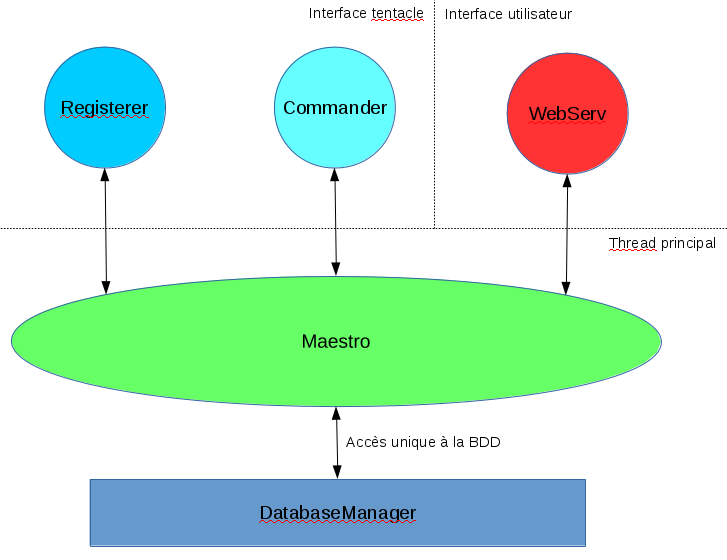
\includegraphics[height=8cm, keepaspectratio=true]{img/algo_brain_full.png}
        \caption{Fonctionnement technique du Brain}
    \end{center} 
\end{figure}

\paragraph{}
L'architecture que nous avons développé pour le Brain reprend une architecture MVC (Modèle-Vue-Contrôleur). Ce type de fonctionnement permet de bien organiser son code source et de séparer facilement les rôles entre les processus du serveur.
Le côté Modèle se retrouve dans le dbManager, la partie Vue est représenté par les différentes interfaces et le Contrôleur correspond au Maestro.

\subsection{Maestro}
\paragraph{}
Le logiciel coté serveur est orchestré autour d'un processus appelé « Maestro ». Son rôle est de coordonner les différents processus que peut lancer le serveur. Ces processus sont des forks permettant de communiquer de manière indépendante avec les clients. 
Le maestro joue un rôle indispensable dans notre logiciel car il est l'interface de communication avec la base de données du serveur. C'est le seul accès permettant de lire et écrire en base de données. En effet, généralement, les bases de données peuvent accepter les accès multiples en lecture mais un accès unique en écriture. Nous avons donc créé ce maestro afin de coordonner tous les liens avec la base de données.
Le maestro est en écoute constante sur des pipes reliés aux différentes parties du serveur. Le contrôle d'accès peut se faire en un point unique grâce à ce Maestro.

\subsection{WebServ}
\paragraph{}
Le WebServ de Octopus permet l’administration du serveur à distance par l’administrateur. 
Ce serveur web permet de voir et d’ajouter les clients, d’envoyer des instructions de scripts aux clients et aussi d’afficher les résultats des scripts éxécutés. 
Le WebServ est l'interface de manipulation des données contenues en base de données. 
\paragraph{}
Le serveur Web est un daemon écrit en C qui permet de lire et d’envoyer des fichiers (HTML, CSS, JavaScript, images) et du texte JSON. 
Le site est formé d'une unique page HTML, dont le contenu est modifié dynamiquement grâce à du javascript et des appels AJAX. 
Les interactions avec des boutons et liens déclenchent des requêtes GET avec différents arguments, et le serveur Web retourne du JSON avec les données demandées. 
Cela permet un contenu dynamique, tout en minimisant les échanges réseau.


\subsection{DbManager, Registerer et Commander}
\paragraph{}
Le DatabaseManager est le gestionnaire de fonctions de lecture et d'écriture dans la base de données. Le logiciel utilise Sqlite3 comme base de données. L'avantage est la facilité d'utilisation de Sqlite3 et il ne demande que peu de ressources matérielles. 
Afin d'accéder en lecture et écriture sur les différentes tables de la base de données, nous avons recréé des fonctions spécifiques.
\paragraph{}
Le Registerer est le daemon d'enregistrement des clients. Il est composé de deux fonctions principales. 
Une première qui est un socket en écoute permanente sur le port 6000 dans le cas ou un Tentacle rejoindrait le réseau et aurait l'adresse IP du Brain. Lorsqu'un nouveau Tentacle tente de contacter le Brain sur le port 6000, celui-ci lance l'enregistrement du Tentacle.
La seconde fonction est appelé lorsque l'administrateur du réseau ajoute manuellement une nouvelle machine sur le réseau. 
L'ajout de la nouvelle machine se fait en fournissant l'adresse IP, ensuite le Brain prend en charge de contacter le client sur le port 7000 pour avoir les informations complémentaires permettant l'enregistrement.
\paragraph{}
Le Commander est le troisième fork qui est en fonctionnement sur le serveur. Celui-ci permet d'envoyer des commandes aux clients et de recevoir les résultats des scripts. 
Ce service se lance lorsque l'administrateur demande à lancer un script sur un Tentacle à travers le WebServ ou quand un Tentacle a terminé l'éxécution d'un script et veut envoyer le résultat de celui-ci au serveur. 
Le Commander peut donc ouvrir une socket vers le client sur le port 7001 pour l'envoi d'une commande, il se déconnecte ensuite. Le Commander est également en écoute sur le port 6001 du Brain et quand un Tentacle se connecte pour envoyer des données, il sauvegarde le rapport en base de données.